\documentclass[titlepage]{jarticle}
\usepackage[dvipdfmx]{graphicx}
\usepackage{listings}
\usepackage{here}
\usepackage{amsmath}
\usepackage[hyphens]{url} % 先にurlパッケージ読込
\usepackage[hidelinks,dvipdfmx]{hyperref}
%高専のstyファイルから拝借
\RequirePackage{geometry,array}

% \zw と \zh の定義
\providecommand{\zw}{zw}
\providecommand{\zh}{zh}

\geometry{left=20mm,right=20mm,top=30mm,bottom=30mm}

\renewcommand{\baselinestretch}{1.25}
%
\lstset{
  basicstyle={\ttfamily},
  identifierstyle={\small},
  % commentstyle={\smallitshape},
  keywordstyle={\small\bfseries},
  ndkeywordstyle={\small},
  stringstyle={\small\ttfamily},
  frame={tb},
  breaklines=true,
  columns=[l]{fullflexible},
  numbers=left,
  xrightmargin=0zw,
  xleftmargin=3zw,
  numberstyle={\scriptsize},
  stepnumber=1,
  numbersep=1zw,
  lineskip=-0.5ex,
  language=java
}
\renewcommand{\lstlistingname}{ソースコード}
\makeatletter
\newcommand{\figcaption}[1]{\def\@captype{figure}\caption{#1}}
\newcommand{\tblcaption}[1]{\def\@captype{table}\caption{#1}}
\makeatother
\begin{document}
\title{測量技術の歴史について}
\author{情報・経営システム工学分野B3\\24336488 本間三暉}
\date{2024年6月26日}
\maketitle
\section{測量の起源と古代エジプトの発展}
測量の起源は紀元前3000年ごろのエジプトにまで遡る.

現在はアスワン・ハイ・ダムが建設されたことによって反乱することのないナイル川だが,
ダムが建設される以前は毎年夏になると季節風という海から陸に向かって湿った風が吹くことによる大量の降水によって必ず河川氾濫していた.
この氾濫により上流にあるエチオピア高原から肥沃な土壌が流れてきて,ほとんど雨が降らないエジプトの農耕と文明の発展を支えた.
このことは人々の生活にも大きな影響を与え,氾濫時期を知るためにシリウス暦が作られ,ナイル川の水位を知るための水位計が各地に設置された.
紀元前3000年ごろのエジプトでは氾濫のたびに区画が破壊されるため,そのたびに区画を作り直すための測量が行われ土地の配分が行われた.
このときに使われたのが,3:4:5の比率で印をつけた縄を張って畑の直角をとり,氾濫で流された農地の境界を復元していた.

ピラミッドの建設では測量技術が使用され,ピラミッドの平均辺長が230.36mに対してピラミッドの最長辺と最短辺の差が20.07cmしかないほど正確に建設されている.
また,ピラミッドの西北隅から東南隅に向かっての勾配は約1.27cmであり,ほぼ水平であることがわかっている.
四隅の直角についての誤差は最大で3.5’(分)であり,辺は真北を向いている.

紀元前2500年頃には水準測定器,垂直確定器,定規といった測量に必要な機器が既に使われていた.
古代エジプトで発達した測量技術はローマ,ギリシア,アラビアへと受け継がれ広まっていった.
\section{地図の始まり}
農耕や建設などの大規模な作業を行われるようになると,大勢の人々の協力が必要になった.バビロニアの粘土板で作られた地図を図\ref{map}に示す.
\begin{figure}[H]
  \centering
  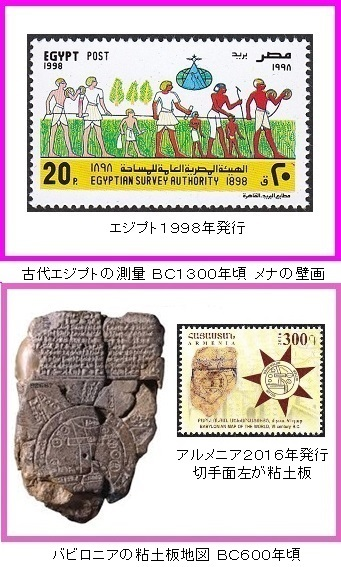
\includegraphics[width=7cm]{img/バビロニア粘土板.jpg}
  \caption{おはよう}
  \label{map}
\end{figure}
aaa

\section*{参考文献}
\begin{enumerate}
  \item 【測量技術の歴史】測量は紀元前3000年のエジプトから存在していた | 東京法経学院 資格コラム\\
        \url{https://www.thg.co.jp/douyo/shikaku/sokuryoshiho/surveying-technique-history/}
  \item モンスーンの意味や定義 わかりやすく解説 Weblio辞書\\
        \url{https://www.weblio.jp/content/モンスーン}
  \item 測量年表\\
        \url{https://www.jsurvey.jp/soknohi/sok-nenpyou.htm}
  \item 測量の歴史 | 大誠色々\\
        \url{http://www.taiseiks.jp/blog_contents_012.html}
  \item
\end{enumerate}
% 
\end{document}